\chapter{Methodology}
\label{chap:methodology}

\lettrine[lines=4, findent=3pt, nindent=0pt]{C}{hapter} 3 deals with software and methodologies used for building the \gls{ids}. Starting with the concept behind the code, will then be discussed the scripts used, the pre-processing done to the chosen dataset, along with some statistics about the latter and the algorithms adopted in the \gls{ml} model training. In the final section will also be provided a \gls{poc} to demonstrate the functioning of the final product. The workflow has revolved around Git as \gls{vcs}\footnote{See section \ref{subsec:repository}}.

%----------------------------------------------------
% CONCEPT
%----------------------------------------------------

\section{Concept}
\label{sec:concept}

In this section will be explained the more abstract and high-level idea, on which the \gls{ids} was built. The concept is summarized by the following figure:

\begin{figure}[h!]
    \centering
    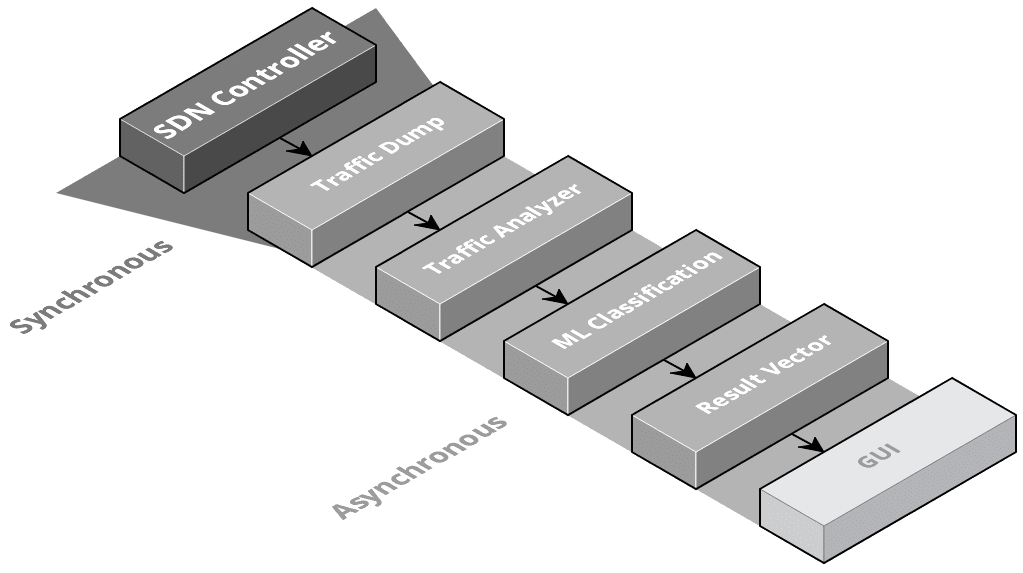
\includegraphics[scale=0.32]{assets/figures/chapter3/concept-components.png}
    \caption{Project's flowchart: from raw traffic to classified vector}
    \label{fig:concept-components}
\end{figure}

\noindent The system can be used in both, \textit{synchronous} or \textit{asynchronous} mode. Proceeding top-down, the \textit{SDN Controller} serves the purpose of orchestrating the duplication of network traffic\footnote{See section \ref{subsubsec:traffic-duplication}} in order to create a \gls{pcap} file (so called \textit{traffic dump}) every some amount of seconds (chosen by the user). The latter will be than passed to the \textit{Analyzer}, which has the task of converting the traffic dump into a vector and pass it to the \gls{ml} model, in order to perform classification. The Analyzer can also get user uploaded files as input, and this allows the asynchronous operation. The \textit{\gls{ml} Classification} block consists of passing the previously mentioned vector to the trained \gls{rf} model and appending periodically the results to a \glsxtrshort{csv} file. In the final step, the \textit{Result Vector} can be visualized using the web \gls{gui}.

%----------------------------------------------------
% MODEL TRAINING
%----------------------------------------------------

\section{Machine Learning Model Training}
\label{sec:model-training}

This is the first stage of the implementation. For this purpose was used a \textit{Jupyter Notebook} to pre-process and visualize the raw data and then to train the \gls{ml} model. For reference, all the operations described were done using a MacBook Pro with 8 GB of RAM and an iMac with 16 GB of RAM, both running macOS 11.4 (Big Sur). The datasets used, as discussed in \ref{subsec:datasets-for-evaluation}, are NSL-KDD and CICIDS2017. The former was only used to become familiar with \gls{ml} and Jupyter Notebooks in general, the latter was the one strictly useful to the project.

%----------------------------------------------------
% PRE-PROCESSING
%----------------------------------------------------

\subsection{Pre-Processing}
\label{subsec:pre-processing}

After the dataset choice, \textit{pre-processing} is very important in order to get consistent results regarding the training of the \gls{ml} model, and so the accuracy of the \gls{ids}. It is important to remove redundant or null records and unimportant features. The dataset used contains plenty records so \texttt{NaN}, \texttt{Null} and \texttt{Inf} values were dropped to clean the data the model will work with. Also columns containing non numerical values were dropped (\texttt{Flow\_ID}, \texttt{Source\_IP}, \texttt{Destination\_IP}, \texttt{Timestamp}), except the one containing the traffic category (\texttt{Label}).
\par Printing the dataset's value counts helps to understand the ratio between normal traffic and malicious one: from table \ref{tab:grouped-dataset-distribution} comes clear that there are traffic categories with insufficient data to train the model, and have to be dropped (\textit{Infiltration}, \textit{SQL Injection} and \textit{Heartbleed}). 

\begin{table}[h!]
    \centering
    \begin{tabular}{l|l}
        \toprule 
        Traffic Label & Entries \\
        \midrule
        \rowcolor{black!10} Benign & 2,271,320 \\
        DoS Hulk & 230,124 \\
        \rowcolor{black!10} Port Scan & 158,804 \\
        DDoS & 128,025 \\
        \rowcolor{black!10} DoS GoldenEye & 10,293 \\
        FTP-Patator & 7,935 \\
        \rowcolor{black!10} SSH-Patator & 5,897 \\
        DoS Slowloris & 5,796 \\
        \rowcolor{black!10} DoS Slowhttptest & 5,499 \\
        Bot & 1,956 \\
        \rowcolor{black!10} Web Attack: Brute Force & 1,507 \\
        Web Attack: XSS & 652 \\
        \rowcolor{black!10} Infiltration & 36 \\
        Web Attack: SQL Injection & 21 \\
        \rowcolor{black!10} Heartbleed & 11 \\
        \bottomrule
    \end{tabular}
    \caption{CICIDS2017 (ungrouped) Value Counts}
    \label{tab:dataset-distribution}
\end{table}

\noindent The remaining 12 labels were then grouped by relevance according to table \ref{tab:grouped-dataset-distribution}, in order to generalize the categorization.

\begin{table}[h!]
    \centering
    \begin{tabular}{l|l|l}
        \toprule 
        Group Name & Labels & Entries \\
        \midrule
        \rowcolor{black!10} Benign & Benign & 2,271,320 \\
        Dos & DoS Hulk, DoS GoldenEye, DoS Slowloris, DoS Slowhttptest &  251,712 \\
        \rowcolor{black!10}Probe & Port Scan & 158,804 \\
        DDoS & DDoS & 128,025 \\
        \rowcolor{black!10}Brute Force & FTP-Patator, SSH-Patator  & 13,832 \\
        Web Attack & Web Attack: Brute Force, Web Attack: XSS & 2,159 \\
        \rowcolor{black!10}Botnet & Bot & 1,956 \\
        \bottomrule
    \end{tabular}
    \caption{CICIDS2017 (grouped) Value Counts}
    \label{tab:grouped-dataset-distribution}
\end{table}

\noindent Another step of the pre-processing stage consisted in splitting the dataset. Being the latter explicitly unbalanced, since it consists in 5 days of traffic acquisition, each one dedicated to a specific attack type, it was performed a \textit{stratified split}, using Pandas' \texttt{train\_test\_split()}, which splits arrays or matrices into train and test subsets, maintaining the same ratio of classes across the subsets. As pointed out in \cite{Mozley2020}, a fundamental step in pre-processing is \textit{normalization}: since the scale of the feature value differs, to ensure that each one of them contribute the same amount to the classification, it is mandatory to bring them to the same range. This kind of operation re-scales the dataset's features using the following equation, in which $x$ is the feature's original value:

\begin{equation}
    x\prime=\frac{x-\min\{x\}}{\max\{x\}-\min\{x\}}
\end{equation}
Many \gls{ml} algorithms perform better when numerical input variables are scaled to a standard range.

%----------------------------------------------------
% FEATURES AND STATISTICS
%----------------------------------------------------

\subsection{Features and Statistics}
\label{subsec:features-statistics}

As pointed out in \ref{subsec:traffic-characterization}, given a dataset, some features are more relevant than others. In order to achieve an higher accuracy and generalization, saving also time in the training stage, the right move was to use only the most relevant features in such a fashion that if the feature value and the class label are independent, then the elder is not relevant to the classification process, therefore it has to be dropped.
\par The tool of choice was the \texttt{SelectKBest} function of the \texttt{scikit-learn} library. This was used to select the top 40 (in this particular case) most dependent features of the dataset, using the \textit{Chi-Square} test which is used to solve the problem in feature selection by testing the relationship between them: it selects the features which are highly dependent on the response. \\ Figure \ref{fig:features-weight} displays a plot of the features score mentioned earlier: the dotted line  represents the $99\%$ mark, meaning that all the features above are not so relevant for the purpose.

\begin{figure}[h!]
    \centering
    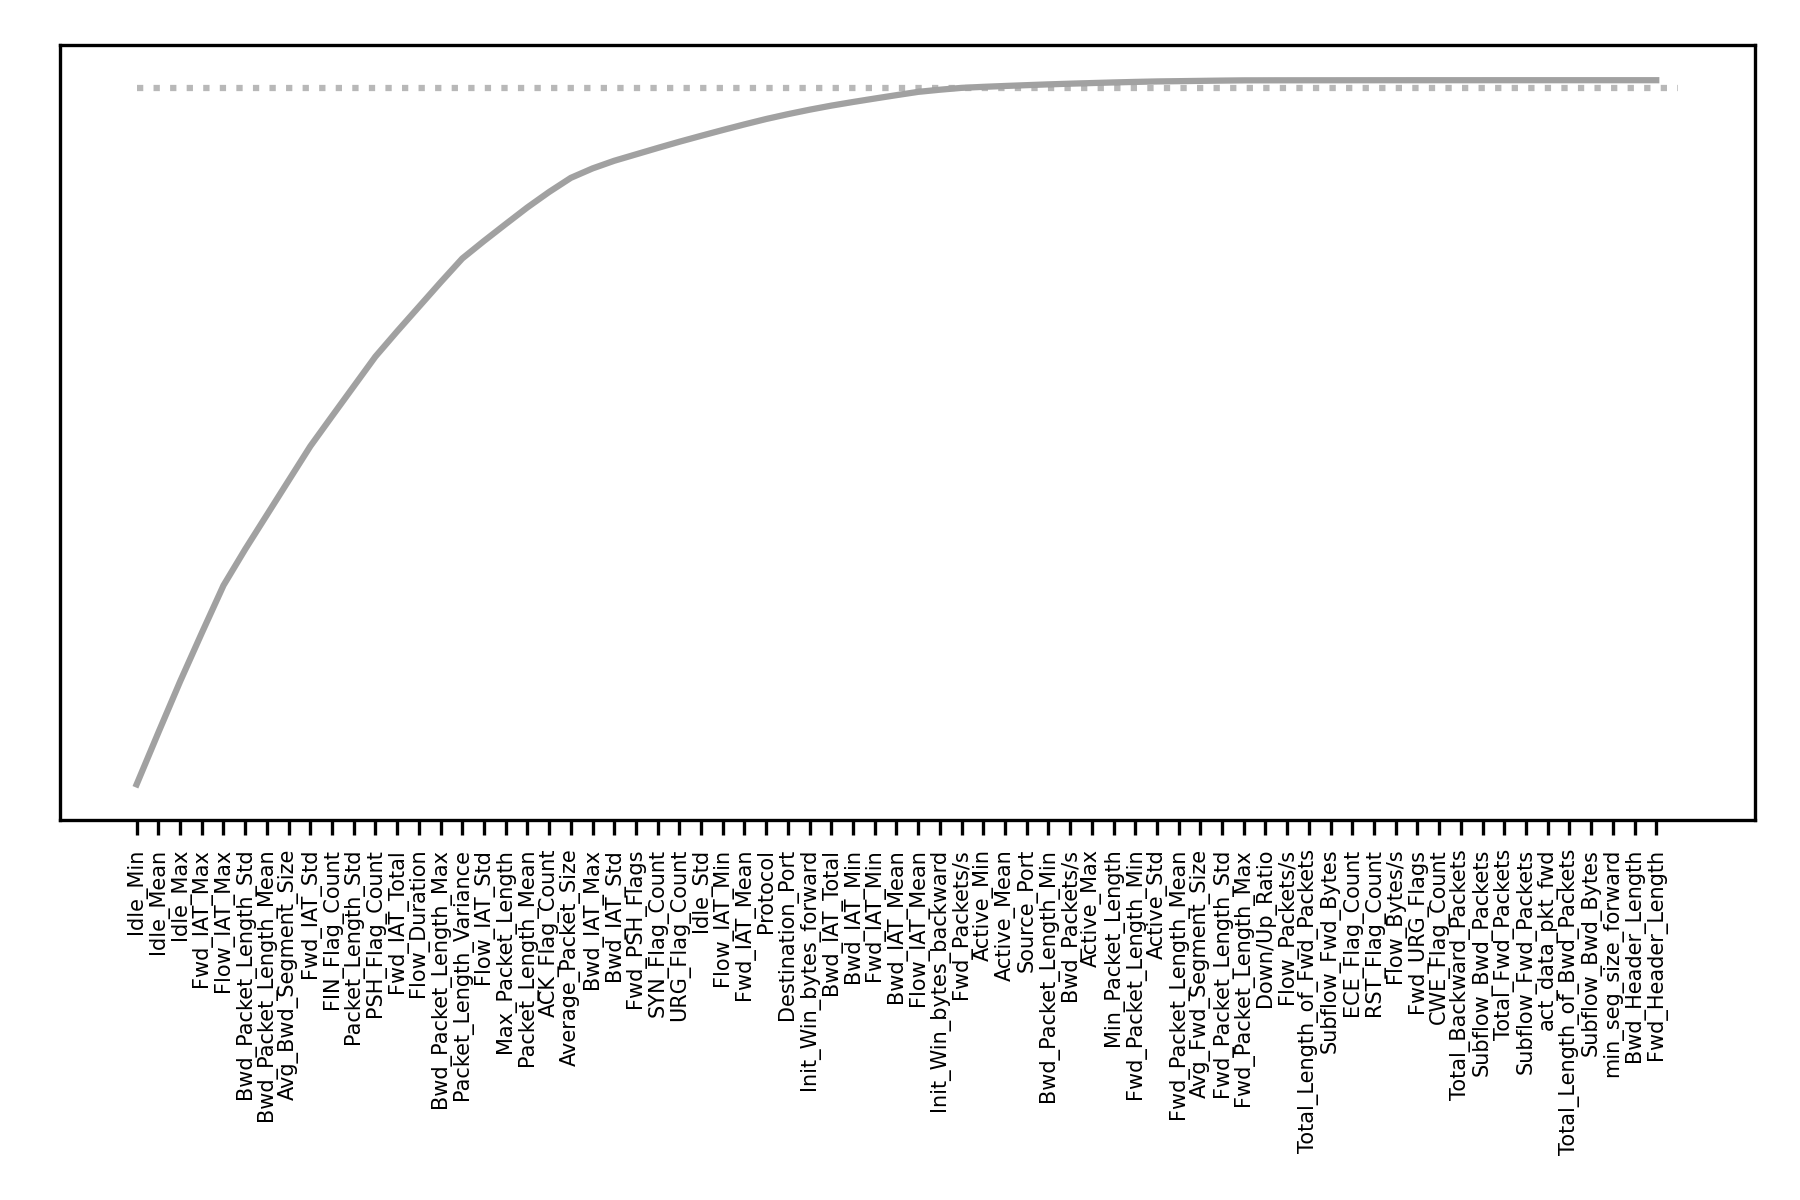
\includegraphics[scale=1]{assets/figures/chapter3/features99.png}
    \caption{CICIDS2017 Features Weight}
    \label{fig:features-weight}
\end{figure}

\noindent To understand which features were used in the training stage, table \ref{tab:features-weight} provides a brief summary. All definitions are drawn from the \textit{CICFlowMeter} project discussed in \cite{icissp17}. \\

\begin{table}[h!]
    \centering
    \begin{tabular}{l|l}
        \toprule 
        Feature & Description \\
        \midrule
        \rowcolor{black!10} \texttt{Destination\_Port} & Destination port number  \\
        \texttt{Protocol} & Protocol used \\
        \rowcolor{black!10} \texttt{Flow\_Duration} & Port Scan \\
        \texttt{Bwd\_Packet\_Length\_Max} & Maximum size of packet in backward direction \\
        \rowcolor{black!10} \texttt{Bwd\_Packet\_Length\_Mean} & Mean size of packet (backward direction) \\
        \texttt{Bwd\_Packet\_Length\_Std} & Standard deviation size of packet (backward direction) \\
        \rowcolor{black!10} \texttt{Flow\_IAT\_Mean} & Mean time between two packets sent in the flow \\
        \texttt{Flow\_IAT\_Std} & Standard deviation time between two packets sent in the flow \\
        \rowcolor{black!10} \texttt{Flow\_IAT\_Max} & Maximum time between two packets sent in the flow \\
        \texttt{Flow\_IAT\_Min} & Minimum time between two packets sent in the flow \\
        \rowcolor{black!10} \texttt{Fwd\_IAT\_Total} & Total time between two packets sent in the forward direction \\
        \texttt{Fwd\_IAT\_Mean} & Mean time between two packets sent in the forward direction \\
        \rowcolor{black!10} \texttt{Fwd\_IAT\_Std} & Standard deviation time between two packets (forward direction) \\
        \texttt{Flow\_IAT\_Max} & Maximum time between two packets sent in the flow \\
        \rowcolor{black!10} \texttt{Flow\_IAT\_Min} & Minimum time between two packets sent in the flow \\
        \texttt{Fwd\_IAT\_Total} & Total time between two packets sent in the forward direction \\
        \rowcolor{black!10} \texttt{Fwd\_IAT\_Mean} & Mean time between two packets (forward direction) \\
        \texttt{Fwd\_IAT\_Std} & Standard deviation time between two packets (forward direction) \\
        \rowcolor{black!10} \texttt{Fwd\_IAT\_Max} & Maximum time between two packets (forward direction) \\
        \texttt{Fwd\_IAT\_Min} & Minimum time between two packets sent in the forward direction \\
        \rowcolor{black!10} \texttt{Bwd\_IAT\_Total} & Total time between two packets (backward direction) \\
        \texttt{Bwd\_IAT\_Mean} & Mean time between two packets sent in the backward direction \\
        \rowcolor{black!10} \texttt{Bwd\_IAT\_Std} & Standard deviation time between two packets (backward direction) \\
        \texttt{Bwd\_IAT\_Max} & Maximum time between two packets sent in the backward direction \\
        \rowcolor{black!10} \texttt{Bwd\_IAT\_Min} & Minimum time between two packets (backward direction) \\
        \texttt{Fwd\_PSH\_Flags} & Number of times the PSH flag was set in packets (forward direction) \\
        \rowcolor{black!10} \texttt{Fwd\_Packets/s} & Number of forward packets per second \\
        \texttt{Max\_Packet\_Length} & Maximum length of a packet \\
        \rowcolor{black!10} \texttt{Packet\_Length\_Mean} & Mean length of a packet \\
        \texttt{Packet\_Length\_Std} & Standard deviation length of a packet \\
        \rowcolor{black!10} \texttt{Packet\_Length\_Variance} & Variance length of a packet \\
        \texttt{FIN\_Flag\_Count} & Number of packets with FIN \\
        \rowcolor{black!10} \texttt{SYN\_Flag\_Count} & Number of packets with SYN \\
        \texttt{PSH\_Flag\_Count} & Number of packets with PUSH \\
        \rowcolor{black!10} \texttt{ACK\_Flag\_Count} & Number of packets with ACK \\
        \texttt{URG\_Flag\_Count} & Number of packets with URG \\
        \rowcolor{black!10} \texttt{Average\_Packet\_Size} & Average size of packet \\
        \texttt{Avg\_Bwd\_Segment\_Size} & Average size observed in the backward direction \\
        \rowcolor{black!10} \texttt{Init\_Win\_bytes\_forward} & Total number of bytes sent in initial window (forward direction) \\
        \texttt{Init\_Win\_bytes\_backward} & Total number of bytes sent in initial window (backward direction) \\
        \rowcolor{black!10} \texttt{Active\_Min} & Minimum time a flow was active before becoming idle \\
        \texttt{Idle\_Mean} & Mean time a flow was idle before becoming active \\
        \rowcolor{black!10} \texttt{Idle\_Std} & Standard deviation time a flow was idle before becoming active \\
        \texttt{Idle\_Max} & Maximum time a flow was idle before becoming active \\
        \rowcolor{black!10} \texttt{Idle\_Min} & Minimum time a flow was idle before becoming active \\
        \bottomrule
    \end{tabular}
    \caption{CICIDS2017 (Selected) Features Weight and Description - most relevant to least relevant}
    \label{tab:features-weight}
\end{table}

\noindent It is interesting to notice that the majority of the selected features are linked either to the statistics of the packet length, to the flags or to time related statistics, such as inter-arrival time between packets and active/ idle time.

%----------------------------------------------------
% CLASSIFICATION
%----------------------------------------------------

\subsection{Classification}
\label{subsec:classification}

As disclosed in \ref{subsec:ml-algorithms}, the algorithm of choice for the classification stage was \textit{Random Forest}. Based on previous works, it is a popular solution in classification problems and this is the reason why was adopted: it can be implemented with ease and can work with large datasets with no problem.
\par The pre-processed dataset, after being split, was passed to the algorithm for training and testing. The results can be found in chapter \ref{chap:results}, along with the confusion matrix, the correlation matrix and the related scores.
\par Regarding the practical implementation, it is straightforward: using \texttt{numpy}, \texttt{pickle} and \texttt{sklearn} libraries, it is possible to load the previously trained model and use it to \textit{predict} a result based on the features vector passed to the \textit{classify} function in \texttt{analyzer.py}.

\begin{figure}[h!]
    \begin{code}[colback=white]{\texttt{Analyzer.py}}{35}
def classify(features):
print('Classifying...')
f = features
features = [[np.nan if x in [np.inf, -np.inf]
                else float(x) for x in features]]

if np.nan in features:
    return

features = normalisation.transform([features])
result = loaded_model.predict(features)

feature_string = [str(i) for i in f]
classification = [str(result[0])]
\end{code}
\end{figure}

\noindent The outcome is then saved in a \gls{csv} file, for later use, such as charts and calculation of further statistics, useful for the \gls{gui} or even future add-ons. 

%----------------------------------------------------
% NETWORK MONITOR
%----------------------------------------------------

\section{Network Monitor}
\label{sec:monitor-implementation}

The \textit{network monitor} is a key component of the system: it is used in both asynchronous and synchronous mode for analyzing the acquired packets, passing them to the model previously discussed. At this point the concept of \textit{flow} discussed in \ref{subsec:network-monitoring} comes in handy.

%----------------------------------------------------
% ML INTEGRATION
%----------------------------------------------------

\subsection{Flow Analysis}
\label{subsec:flow-analysis}

The \textit{Transport Layer} protocols relevant for the implementation are \gls{tcp} and \gls{udp}. As considered in \cite{Mozley2020}, \gls{udp} flows terminate on \textit{time out}, while \gls{udp} ones end with a \textit{time out}, but may also terminate via the \texttt{FIN} flag (last packet from sender), or \texttt{RST} flag (connection reset). The first packet in the flow is assumed to be in the forward direction, defining the source and, accordingly, the traffic directions.
\par The code snippet below (from \texttt{analyzer.py}) displays how packet reception is handled: if a packet doesn't belong to an existing flow, a new flow instance is created, otherwise it is necessary to check if it is a terminating packet. All current flows are stored in a dictionary, with the keys being the \textit{flow-ID}, and the value is the reference to the flow object. The features previously discussed are calculated after the flow is terminated and then passed to the classified in a \textit{feature vector}. The Python library of choice for the feature extraction was \texttt{Scapy} \cite{ScapyLibrary}: a packet manipulation program able to decode packets of a wide number of protocols. The retrieved information was then passed to the \textit{statistics} module in order to calculate features to include in the vector.

\begin{figure}[h!]
    \begin{code}[colback=white]{\texttt{Analyzer.py}}{92}
if packet.getFwdID() in current_flows.keys():
  flow = current_flows[packet.getFwdID()]
  if (packet.getTimestamp() - flow.getFlowStartTime()) > FlowTimeout:
    classify(flow.terminated())
    del current_flows[packet.getFwdID()]
    flow = Flow(packet)
    current_flows[packet.getFwdID()] = flow
  elif packet.getFINFlag() or packet.getRSTFlag():
    flow.new(packet, 'fwd')
    classify(flow.terminated())
    del current_flows[packet.getFwdID()]
    del flow
  else:
    flow.new(packet, 'fwd')
    current_flows[packet.getFwdID()] = flow
elif packet.getBwdID() in current_flows.keys():
  flow = current_flows[packet.getBwdID()]
  if (packet.getTimestamp() - flow.getFlowStartTime()) > FlowTimeout:
    classify(flow.terminated())
    del current_flows[packet.getBwdID()]
    del flow
    flow = Flow(packet)
    current_flows[packet.getFwdID()] = flow
  elif packet.getFINFlag() or packet.getRSTFlag():
    flow.new(packet, 'bwd')
    classify(flow.terminated())
    del current_flows[packet.getBwdID()]
    del flow
  else:
    flow.new(packet, 'bwd')
    current_flows[packet.getBwdID()] = flow
else:
  flow = Flow(packet)
  current_flows[packet.getFwdID()] = flow
    \end{code}
\end{figure}

%----------------------------------------------------
% SDN MONITOR
%----------------------------------------------------

\subsection{SDN Monitor}
\label{subsec:sdn-monitor}

As mentioned above, the \gls{sdn} implementation relies on \textit{Ryu Controller}: to create a \gls{tap} like setup, a switch script was modified to work at level 3 of the \textit{TCP/IP Stack}, saving all the traffic passing through it in a \gls{pcap} file. The network dump can then be analysed instantly or saved for later use, as needed.
\par To achieve the tool of choice was, the \texttt{pcaplib} module of \texttt{ryu} library: adding few lines of code to the \texttt{\_packet\_in\_handler()} function of the switch allowed to save the traffic passing through it in files named after the timestamp. This feature can then be implemented, as did in the \texttt{Flask} application discussed in \ref{sec:poc}, using Python's \texttt{subprocess} library to run several instances at the same time.

%----------------------------------------------------
% POC
%----------------------------------------------------

\section{Proof of Concept}
\label{sec:poc}

As expressed at the beginning of the dissertation, one of the objectives was to create a \gls{poc} of what could be a commercial product.
\par The system is designed to be modular and can be adapted to the deploying scenario, as needed. Figure \ref{fig:gui-mockup} shows the app created using a micro-framework written in Python, named \texttt{Flask} \cite{FlaskLibrary}, that integrates a \gls{gui}, although the \gls{ids} can be used from the command line, remaining fully functional. To summarize, the main components of the application are:

\begin{itemize}
    \itemAR \textit{Network Monitor}: discussed in the previous section, it accepts \gls{pcap} files and classifies their network traffic;
    \itemAR \gls{tap} - \textit{L3 Switch}: has the only function of creating the \gls{pcap} files to pass to the monitor;
    \itemAR \textit{Dashboard}: it gives useful information, such as the disk space used by the network dumps (which can be limited), the classification results and can be integrated with other metrics and charts.
\end{itemize}
All three can work standalone, but they are brought together by the Flask implementation of the project.

%----------------------------------------------------
% GUI
%----------------------------------------------------

\subsection{Graphical User Interface}
\label{subsec:gui}

As just mentioned, the \gls{gui} unifies the components and makes it easier, for example, to choose between \textit{synchronous} and \textit{asynchronous} mode, or to set the maximum disk space to allocate for the traffic acquisition.

\begin{figure}[h!]
    \centering
    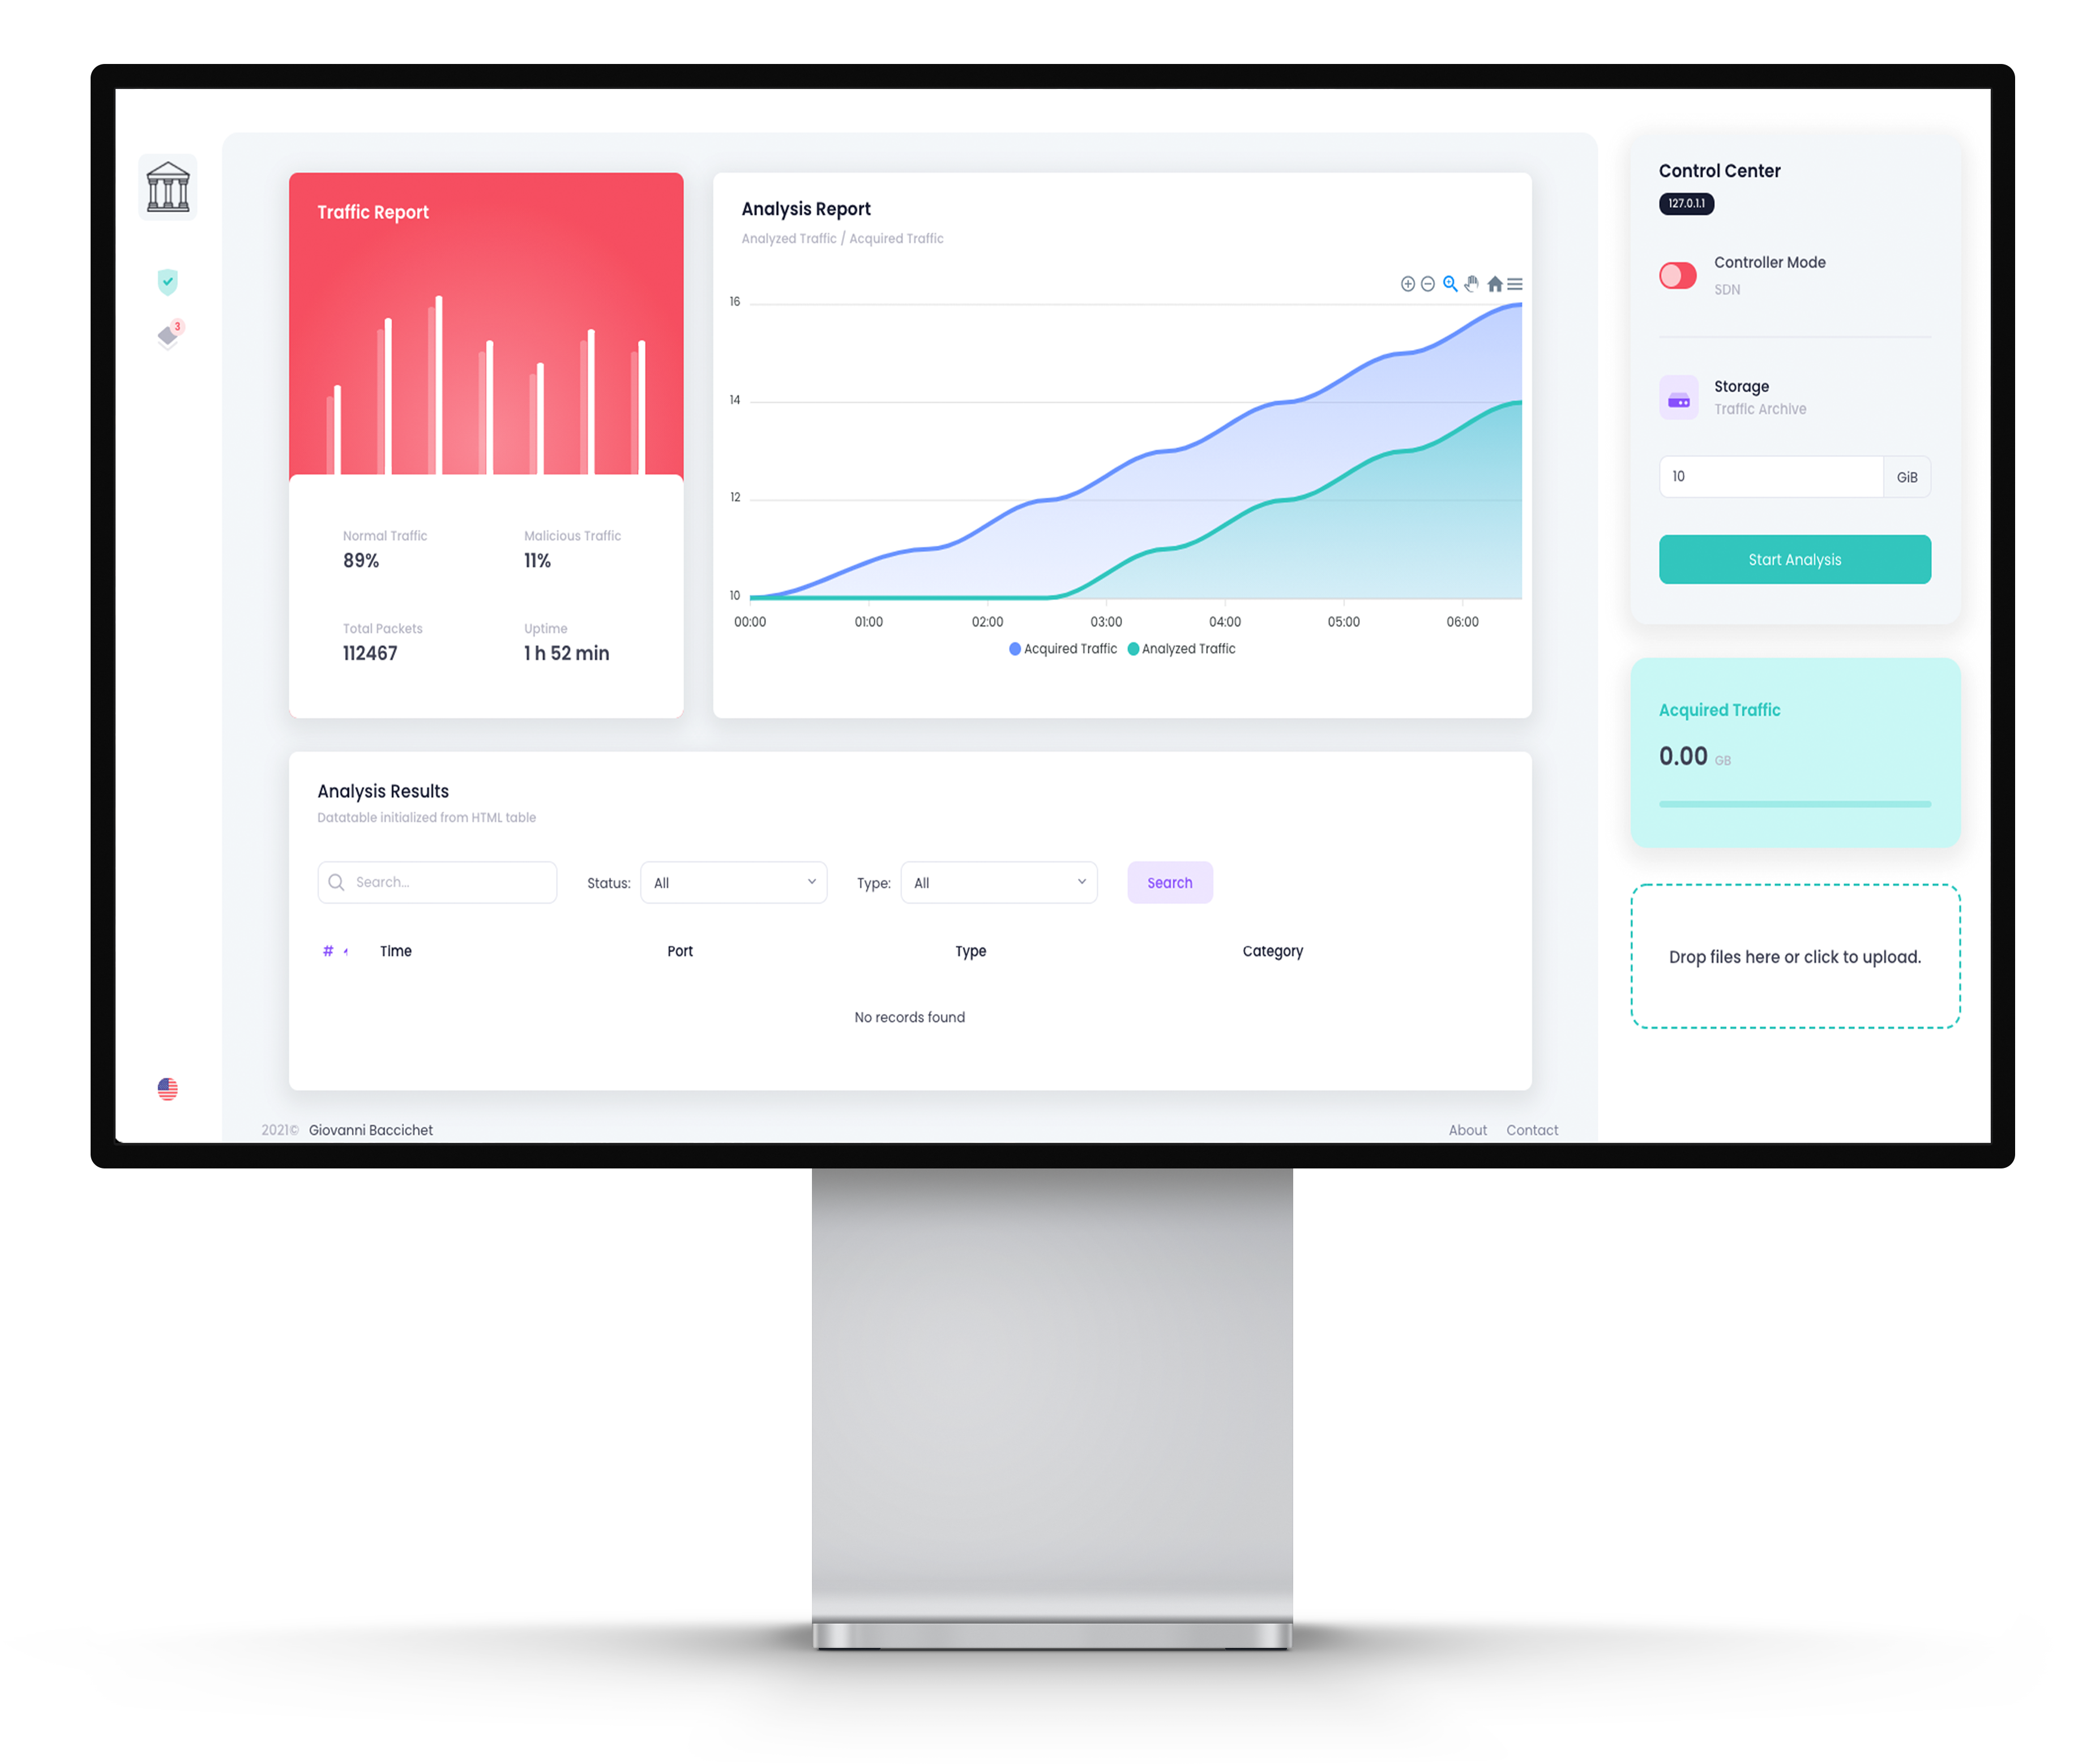
\includegraphics[scale=0.4]{assets/figures/chapter3/gui-mockup.png}
    \caption{Flask implementation of the \gls{gui}}
    \label{fig:gui-mockup}
\end{figure}

\par The \textit{back-end} is built using \texttt{Flask}, while the \textit{front-end} uses \textit{Bootstrap} \cite{BootstrapLibrary} with a custom graphic. The controls, such as the toggle switch for the \textit{SDN mode} (\textit{synchronous mode}), the input for the maximum storage, etc. are sent to the \textit{back-end} through \gls{ajax}, in oder to be interactive and exchange data in the background, without refreshing the web page after every modification of said parameters.

\subsubsection{Functions and Add-Ons}
\label{subsubsec:functions}

While designing the \gls{gui}, the one feature to keep in mind was expandability: building a dashboard with more functions than necessary was a nonsense. For this reason the modules concerning metrics and data (the ones in the center portion of the screen) can be modified and replaced with different or new ones: they all use \gls{ajax} and the \texttt{Flask} app, equipped with the \texttt{jsonify} library can easily send \gls{ajax} responses to the \gls{gui}, containing the desired information. In other words, \textit{add-ons} can be created with ease and integrated into the deploying environment, keeping in mind that Python provides endless solution for data manipulation, on the \textit{back-end}.
\par The labels containing system information are also managed by the Python \textit{back-end}, using the \texttt{socket} library for gathering the IP address of the machine, the \texttt{os} and \texttt{pathlib} libraries for calculating the remaining space on the disk.
\par Upload is managed by the \texttt{Dropzone} module of the \texttt{flask\_dropzone} library: it allows for an easy implementation of the drag and drop functionality, with file format and file size controls; in fact only \gls{pcap} files can be uploaded.

%----------------------------------------------------
% TOPOLOGY
%----------------------------------------------------

\subsection{Topology and Testing}
\label{subsec:topology}

Some of the perks of \gls{sdn} paradigm are scalability and flexibility: figure \ref{fig:poc-topology} represents a very simple network topology created using \textit{mininet} to test the \gls{ids} capabilities on a realistic environment. A remarkable fact is that both the controller and the \gls{ids}, as shown, can be in a remote location: this feature is appealing and relevant for modern applications since they both can be virtualized in the cloud, allowing for more flexibility at a lower cost.

\begin{figure}[h!]
    \centering
    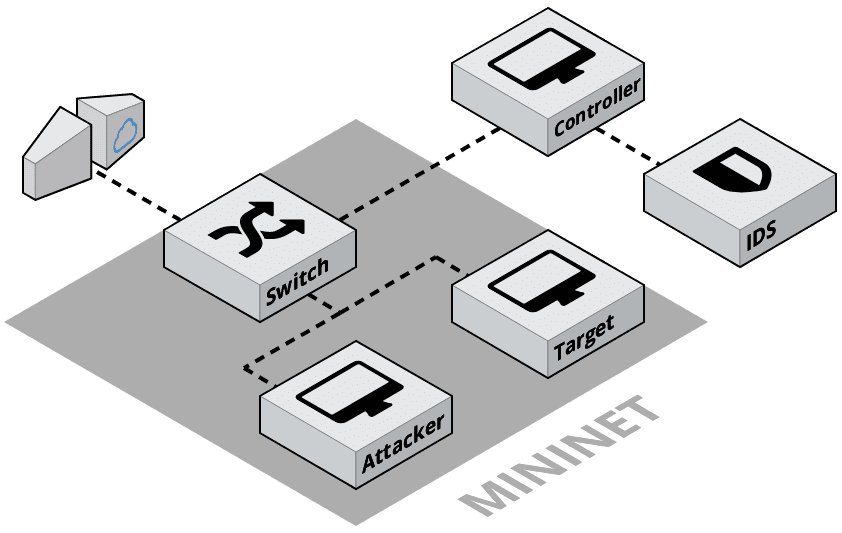
\includegraphics[scale=0.25]{assets/figures/chapter3/PoC_topology.png}
    \caption{Proof of Concept - Example of simple tree topology using \textit{mininet}}
    \label{fig:poc-topology}
\end{figure}
Another way of testing the \gls{ids} capabilities is by using its \textit{asynchronous mode}: practically uploading a \gls{pcap} file to the web interface and checking if the results meet the expectations. Obviously said traffic dump has to be acquired in a controlled environment in order to be able to have a precise idea on the type of traffic and the related classification.

%----------------------------------------------------
% ATTACK TOOLS
%----------------------------------------------------

\subsection{Penetration Testing Tools}
\label{subsec:pentesting-tools}
\textcolor{dimgray}{\lipsum[1]}

% \subsubsection{Stress Testing}
% \label{subsubsec:stress-testing}
% \textcolor{dimgray}{\lipsum[1]}

% \subsubsection{Password Attacks}
% \label{subsubsec:password-attacks}
% \textcolor{dimgray}{\lipsum[1]}

% \subsubsection{Information Gathering}
% \label{subsubsec:information-gathering}
% \textcolor{dimgray}{\lipsum[1]}

% \subsubsection{Web Applications}
% \label{subsubsec:web-applications}
% \textcolor{dimgray}{\lipsum[1]}

%----------------------------------------------------
% REPOSITORY OVERVIEW
%----------------------------------------------------

\newpage

\subsection{Repository Overview}
\label{subsec:repository}

This repository is available on GitHub [{\fontsize{7}{7}\faExternalLink*[regular]} \href{https://github.com/GiovanniBaccichet/themis/}{\texttt{github.com/GiovanniBaccichet/themis}}].
\par Summarizing what mentioned in the above sections, the first stage of this work consisted in the dataset pre-processing and the \gls{ml} model training: relevant files can be found in the \texttt{Jupyter Notebook/} folder, more specifically, the \texttt{FlowMeter Training/} subdirectory contains what was used in the final implementation, while \texttt{NSL-KDD Training/} contains first attempts of data manipulation and \gls{ml} training.
\par The second stage concerned developing the network monitor and the network \gls{tap}; the respective files can be found in \texttt{app/} and \texttt{SDN/}.
\par Lastly, all the components are brought together by the flask app named \texttt{themis.py}: the directories related to the web application are \texttt{static/} and \texttt{templates/}, while the other folders contain, as discussed above, all the components relevant to the traffic acquisition and \gls{ml} classification. 

\begin{figure}[h!]
    \centering
    \begin{forest}
        for tree={
          font=\ttfamily,
          grow'=0,
          folder,
          l sep=20pt,
          edge path={
        \noexpand\path [draw, \forestoption{edge}] (!u.parent anchor) ++(1em,0) |- node[fill,inner sep=0pt] {} (.child anchor)\forestoption{edge label};
      },
          if n children=0{
            before typesetting nodes={
              tempdima=\iconsepfrompath+\iconsep+6*\touchsize,
              content/.wrap value={\expandafter\hskip \foresteregister{tempdima}#1},
            },
            tikz={%
              \pic [xshift=\iconsepfrompath] at (.west) {touch};
            },
          }{
            if level=0{
              tikz={%
                \pic [xshift=\iconsepfrompath] at (.west) {mkdir};
              },
              before typesetting nodes={
                tempdima=\iconsep+12*\mkdirsize,
                content/.wrap value={\expandafter\hskip \foresteregister{tempdima}#1},
              },
            }{
              tikz={%
                \pic [xshift=\iconsepfrompath] at (.west) {mkdir};
              },
              before typesetting nodes={
                tempdima=\iconsepfrompath+\iconsep+10*\mkdirsize,
                content/.wrap value={\expandafter\hskip \foresteregister{tempdima}#1},
              },
            },
          },
        },
        [themis, optional
          [app
            [analyzer.py]
            [features.py]
            [flow.py]
            [pktInfo.py]
          ]
          [Jupyter Notebook
            [FlowMeter Training
            [FlowMeter Training.ipynb]
            [Models
            [grouped\_model.pickle]
            [ungrouped\_model.pickle]
            ]
            ]
            [NSL-KDD Training
            [NSL-KDD Training.ipynb]
            ]
          ]
          [SDN
            [L3\_switch.py]
          ]
          [templates
          [index.html]
          ]
          [requirements.txt]
          [themis.py]
        ]
      \end{forest}
    \caption{Structure of Source Code Repository}
    \label{fig:repository-structure}
\end{figure}

Some files are omitted: all \texttt{.csv} and \texttt{.pcap} files are in the \texttt{.gitignore} for privacy reasons, so the datasets used are not directly available, but can be downloaded from the respective websites. The application's output is saved in \gls{csv} format in order to be reviewed at a later time, for this reason it will not be in this repository out of the box, but has to be generated by the user.